\section{Overview}\label{sec:overview}

The housing subsidy scenario in \autoref{sec:motivation} exhibits both types of cross-layer design error the formalization detects: a vertical governance conflict on a single credential's format assignment, and a horizontal capability gap spanning two credentials (\autoref{sec:headlines}). \autoref{sec:functional-overview} defines the three usage modes the framework must support.

\subsection{Motivation}\label{sec:motivation}

Consider a government housing subsidy where eligibility requires credentials from three independent authorities: family status from a civil registry, property records from a land registry, and income from an employer.\footnote{Based on the Hungarian Family Housing Subsidy (Családi Otthonteremtési Kedvezmény, CSOK), simplified. Additional credentials required in practice (tax clearance, criminal record check) are omitted; these involve simple status checks that do not introduce cross-credential arithmetic or predicate proof requirements, and their inclusion would not affect the headline results.} The required property size depends on the number of children \citep{noauthor_5182023_2023} (the decree prescribes minimum floor areas of 40, 50, 60, 70, and 80 m² for one through five or more children, respectively), a constraint that spans two credentials, and the income check must satisfy both EU format mandates and data protection requirements.

\autoref{fig:teaser} illustrates this scenario across three metamodel layers. At the domain concept layer, the applicant's facts (number of children, property floor area, monthly income) form an information graph with domain-level constraints: the minimum floor area is a function of the number of children \citep{noauthor_5182023_2023}, and income must exceed a regulatory threshold. At the credential schema layer, these facts are distributed across three credentials issued by independent authorities, each with its own credential subject. All three subjects must be aligned (they refer to the same applicant) and each claim must trace to the corresponding domain-level property. At the format-specific layer, EU regulations mandate specific credential formats for government-issued attestations \citep{noauthor_eu-digital-identity-walleteudi-doc-architecture-and-reference-framework_2026}, while data protection law's minimization principle, operationalized here as a credential-layer requirement, implies that privacy-sensitive checks such as whether income exceeds a threshold should not require disclosing the underlying value \citep{gdpr}.\footnote{A directly analogous enforcement action supports this operationalization: the Hungarian data protection authority (NAIH) fined a bank 35M HUF for copying applicants' entire pregnancy booklets when only a 12-week gestation threshold check was required for a subsidized loan, finding the collection grossly disproportionate \citep{noauthor_naih_2020}.}

Inspected in isolation, each layer is well-formed: domain properties, credential schemas, and format assignments each pass their own validation. Cross-layer analysis, however, reveals two problems. The income credential cannot simultaneously satisfy the eIDAS \ac{ARF} format mandate (requiring SD-JWT-VC \citep{noauthor_eu-digital-identity-walleteudi-doc-architecture-and-reference-framework_2026}) and \ac{GDPR} data minimization (requiring predicate proof capability \citep{gdpr}); SD-JWT-VC supports selective disclosure but not predicate proofs. The floor area constraint requires cross-credential predicate evaluation spanning two credentials, which no widely used format supports in zero-knowledge. Neither problem is visible when any single layer is inspected alone.

The constraints in this scenario originate from governance frameworks that were not designed to be jointly satisfied: W3C VCDM \citep{sporny_verifiable_2025} defines structural conformance rules for credentials, the eIDAS \ac{ARF} \citep{noauthor_eu-digital-identity-walleteudi-doc-architecture-and-reference-framework_2026} mandates specific credential formats for government attestations, \ac{GDPR} \citep{gdpr} requires data minimization, and format specifications \citep{terbu_sd-jwt-based_2026, curran2022anoncreds} define what each format can and cannot express. These sources were enacted independently; no single source anticipates the constraints imposed by the others.

The remainder of this section defines a framework that captures constraints across these layers and governance sources and demonstrates how it can be used by a designer.

\begin{figure*}[t]
  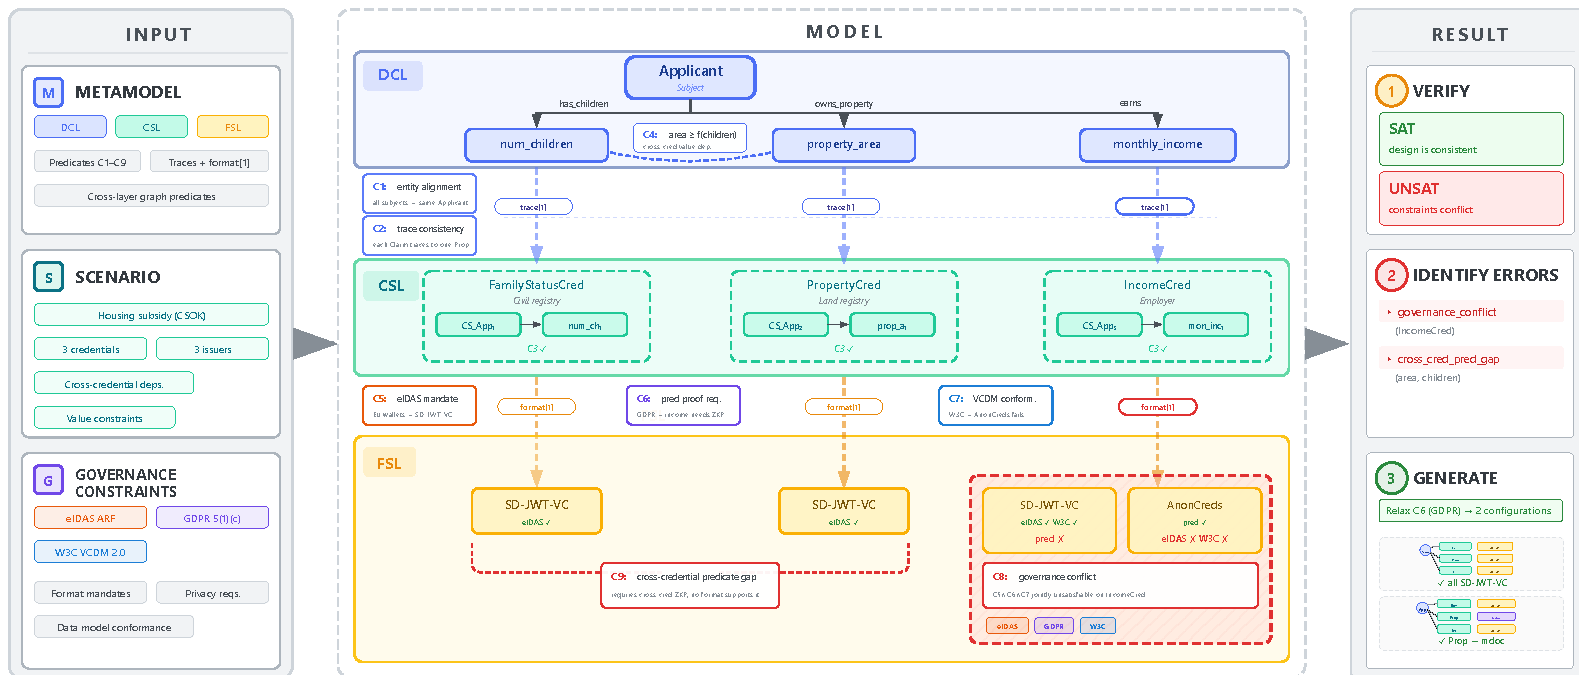
\includegraphics[width=\textwidth]{assets/teaser.pdf}
  \caption{The proposed multi-layer modeling framework applied to a housing subsidy credential ecosystem across three metamodel layers, from domain facts through credential schemas to format-specific representations. Error identification detects conflicting governance requirements on the income credential; design space exploration confirms no valid format assignment exists. Both results require cross-layer analysis.}
  \Description{Teaser figure description.}
  \label{fig:teaser}
\end{figure*}

\subsection{Functional Overview}\label{sec:functional-overview}

\autoref{fig:teaser} illustrates the framework on the housing subsidy scenario. A credential ecosystem designer provides a \emph{partial design}: the ecosystem's entities, credentials, and their relationships, together with governance constraints from regulatory and technical sources. Some choices, such as format assignments, may be left open for the framework to resolve. The metamodel (\autoref{sec:approach}) organizes design elements across three layers, and cross-layer constraints, expressed as graph predicates, are evaluated by the Refinery partial graph modeling framework \citep{marussy_refinery_2024}.

The framework supports three usage modes. \emph{Consistency checking} confirms that a complete design satisfies all constraints. \emph{Error identification} pinpoints which constraints conflict and where; in the housing subsidy scenario, it reports that the income credential's format assignment simultaneously violates a governance mandate and a data protection requirement (\autoref{fig:teaser}). When the designer leaves choices open, \acf{DSE} generates diverse valid completions\footnote{Refinery's diversity mechanism yields meaningfully distinct graph completions; the designer inspects a representative sample rather than an exhaustive enumeration.} or proves that no satisfying configuration exists. A typical workflow chains these modes: the designer runs error identification to discover the income credential conflict, restructures the income claim as a pre-computed boolean, then runs \ac{DSE} to search for valid format assignments.
